
%% bare_jrnl.tex
%% V1.4b
%% 2015/08/26
%% by Michael Shell
%% see http://www.michaelshell.org/
%% for current contact information.
%%
%% This is a skeleton file demonstrating the use of IEEEtran.cls
%% (requires IEEEtran.cls version 1.8b or later) with an IEEE
%% journal paper.
%%
%% Support sites:
%% http://www.michaelshell.org/tex/ieeetran/
%% http://www.ctan.org/pkg/ieeetran
%% and
%% http://www.ieee.org/

%%*************************************************************************
%% Legal Notice:
%% This code is offered as-is without any warranty either expressed or
%% implied; without even the implied warranty of MERCHANTABILITY or
%% FITNESS FOR A PARTICULAR PURPOSE! 
%% User assumes all risk.
%% In no event shall the IEEE or any contributor to this code be liable for
%% any damages or losses, including, but not limited to, incidental,
%% consequential, or any other damages, resulting from the use or misuse
%% of any information contained here.
%%
%% All comments are the opinions of their respective authors and are not
%% necessarily endorsed by the IEEE.
%%
%% This work is distributed under the LaTeX Project Public License (LPPL)
%% ( http://www.latex-project.org/ ) version 1.3, and may be freely used,
%% distributed and modified. A copy of the LPPL, version 1.3, is included
%% in the base LaTeX documentation of all distributions of LaTeX released
%% 2003/12/01 or later.
%% Retain all contribution notices and credits.
%% ** Modified files should be clearly indicated as such, including  **
%% ** renaming them and changing author support contact information. **
%%*************************************************************************


% *** Authors should verify (and, if needed, correct) their LaTeX system  ***
% *** with the testflow diagnostic prior to trusting their LaTeX platform ***
% *** with production work. The IEEE's font choices and paper sizes can   ***
% *** trigger bugs that do not appear when using other class files.       ***                          ***
% The testflow support page is at:
% http://www.michaelshell.org/tex/testflow/



\documentclass[journal]{IEEEtran}
%
% If IEEEtran.cls has not been installed into the LaTeX system files,
% manually specify the path to it like:
% \documentclass[journal]{../sty/IEEEtran}





% Some very useful LaTeX packages include:
% (uncomment the ones you want to load)


% *** MISC UTILITY PACKAGES ***
%
%\usepackage{ifpdf}
% Heiko Oberdiek's ifpdf.sty is very useful if you need conditional
% compilation based on whether the output is pdf or dvi.
% usage:
% \ifpdf
%   % pdf code
% \else
%   % dvi code
% \fi
% The latest version of ifpdf.sty can be obtained from:
% http://www.ctan.org/pkg/ifpdf
% Also, note that IEEEtran.cls V1.7 and later provides a builtin
% \ifCLASSINFOpdf conditional that works the same way.
% When switching from latex to pdflatex and vice-versa, the compiler may
% have to be run twice to clear warning/error messages.






% *** CITATION PACKAGES ***
%
%\usepackage{cite}
% cite.sty was written by Donald Arseneau
% V1.6 and later of IEEEtran pre-defines the format of the cite.sty package
% \cite{} output to follow that of the IEEE. Loading the cite package will
% result in citation numbers being automatically sorted and properly
% "compressed/ranged". e.g., [1], [9], [2], [7], [5], [6] without using
% cite.sty will become [1], [2], [5]--[7], [9] using cite.sty. cite.sty's
% \cite will automatically add leading space, if needed. Use cite.sty's
% noadjust option (cite.sty V3.8 and later) if you want to turn this off
% such as if a citation ever needs to be enclosed in parenthesis.
% cite.sty is already installed on most LaTeX systems. Be sure and use
% version 5.0 (2009-03-20) and later if using hyperref.sty.
% The latest version can be obtained at:
% http://www.ctan.org/pkg/cite
% The documentation is contained in the cite.sty file itself.






% *** GRAPHICS RELATED PACKAGES ***
%
\ifCLASSINFOpdf
\usepackage[pdftex]{graphicx}
% declare the path(s) where your graphic files are
%\graphicspath{{../pdf/}{../jpeg/}}
\graphicspath{{images/}}
% and their extensions so you won't have to specify these with
% every instance of \includegraphics
% \DeclareGraphicsExtensions{.pdf,.jpeg,.png}
\else
% or other class option (dvipsone, dvipdf, if not using dvips). graphicx
% will default to the driver specified in the system graphics.cfg if no
% driver is specified.
% \usepackage[dvips]{graphicx}
% declare the path(s) where your graphic files are
% \graphicspath{{../eps/}}
% and their extensions so you won't have to specify these with
% every instance of \includegraphics
% \DeclareGraphicsExtensions{.eps}
\fi
% graphicx was written by David Carlisle and Sebastian Rahtz. It is
% required if you want graphics, photos, etc. graphicx.sty is already
% installed on most LaTeX systems. The latest version and documentation
% can be obtained at: 
% http://www.ctan.org/pkg/graphicx
% Another good source of documentation is "Using Imported Graphics in
% LaTeX2e" by Keith Reckdahl which can be found at:
% http://www.ctan.org/pkg/epslatex
%
% latex, and pdflatex in dvi mode, support graphics in encapsulated
% postscript (.eps) format. pdflatex in pdf mode supports graphics
% in .pdf, .jpeg, .png and .mps (metapost) formats. Users should ensure
% that all non-photo s use a vector format (.eps, .pdf, .mps) and
% not a bitmapped formats (.jpeg, .png). The IEEE frowns on bitmapped formats
% which can result in "jaggedy"/blurry rendering of lines and letters as
% well as large increases in file sizes.
%
% You can find documentation about the pdfTeX application at:
% http://www.tug.org/applications/pdftex





% *** MATH PACKAGES ***
%
\usepackage{amsmath}
%\usepackage{calrsfs}
%\usepackage{bm}
\usepackage{amssymb}
\usepackage{array}
\usepackage{tabu}
\usepackage{float}
\usepackage{svg}
%\usepackage[]{algorithm2e}
%\usepackage{algorithm}
%\usepackage[]{algorithmic}
\usepackage{algorithm, algorithmic}
%\usepackage[colorlinks]{hyperref}
\usepackage{xcolor}

\usepackage[nottoc]{tocbibind}
\newcolumntype{M}[1]{>{\centering\arraybackslash}m{#1}}
\newcolumntype{N}{@{}m{0pt}@{}}


\newcommand\norm[1]{\left\lVert#1\right\rVert}

\newcommand{\trans}{\mathsf{T}}



%\DeclareMathAlphabet{\pazocal}{OMS}{zplm}{m}{n}
% A popular package from the American Mathematical Society that provides
% many useful and powerful s for dealing with mathematics.
%
% Note that the amsmath package sets \interdisplaylinepenalty to 10000
% thus preventing page breaks from occurring within multiline equations. Use:
%\interdisplaylinepenalty=2500
% after loading amsmath to restore such page breaks as IEEEtran.cls normally
% does. amsmath.sty is already installed on most LaTeX systems. The latest
% version and documentation can be obtained at:
% http://www.ctan.org/pkg/amsmath






% *** SPECIALIZED LIST PACKAGES ***
%
%\usepackage{algorithmic}
% algorithmic.sty was written by Peter Williams and Rogerio Brito.
% This package provides an algorithmic environment fo describing algorithms.
% You can use the algorithmic environment in-text or within a figure
% environment to provide for a floating algorithm. Do NOT use the algorithm
% floating environment provided by algorithm.sty (by the same authors) or
% algorithm2e.sty (by Christophe Fiorio) as the IEEE does not use dedicated
% algorithm float types and packages that provide these will not provide
% correct IEEE style captions. The latest version and documentation of
% algorithmic.sty can be obtained at:
% http://www.ctan.org/pkg/algorithms
% Also of interest may be the (relatively newer and more customizable)
% algorithmicx.sty package by Szasz Janos:
% http://www.ctan.org/pkg/algorithmicx




% *** ALIGNMENT PACKAGES ***
%
%\usepackage{array}
% Frank Mittelbach's and David Carlisle's array.sty patches and improves
% the standard LaTeX2e array and tabular environments to provide better
% appearance and additional user controls. As the default LaTeX2e table
% generation code is lacking to the point of almost being broken with
% respect to the quality of the end results, all users are strongly
% advised to use an enhanced (at the very least that provided by array.sty)
% set of table tools. array.sty is already installed on most systems. The
% latest version and documentation can be obtained at:
% http://www.ctan.org/pkg/array


% IEEEtran contains the IEEEeqnarray family of commands that can be used to
% generate multiline equations as well as matrices, tables, etc., of high
% quality.




% *** SUBFIGURE PACKAGES ***
%\ifCLASSOPTIONcompsoc
%  \usepackage[caption=false,font=normalsize,labelfont=sf,textfont=sf]{subfig}
%\else
%  \usepackage[caption=false,font=footnotesize]{subfig}
%\fi
% subfig.sty, written by Steven Douglas Cochran, is the modern replacement
% for subfigure.sty, the latter of which is no longer maintained and is
% incompatible with some LaTeX packages including fixltx2e. However,
% subfig.sty requires and automatically loads Axel Sommerfeldt's caption.sty
% which will override IEEEtran.cls' handling of captions and this will result
% in non-IEEE style figure/table captions. To prevent this problem, be sure
% and invoke subfig.sty's "caption=false" package option (available since
% subfig.sty version 1.3, 2005/06/28) as this is will preserve IEEEtran.cls
% handling of captions.
% Note that the Computer Society format requires a larger sans serif font
% than the serif footnote size font used in traditional IEEE formatting
% and thus the need to invoke different subfig.sty package options depending
% on whether compsoc mode has been enabled.
%
% The latest version and documentation of subfig.sty can be obtained at:
% http://www.ctan.org/pkg/subfig




% *** FLOAT PACKAGES ***
%
%\usepackage{fixltx2e}
% fixltx2e, the successor to the earlier fix2col.sty, was written by
% Frank Mittelbach and David Carlisle. This package corrects a few problems
% in the LaTeX2e kernel, the most notable of which is that in current
% LaTeX2e releases, the ordering of single and double column floats is not
% guaranteed to be preserved. Thus, an unpatched LaTeX2e can allow a
% single column figure to be placed prior to an earlier double column
% figure.
% Be aware that LaTeX2e kernels dated 2015 and later have fixltx2e.sty's
% corrections already built into the system in which case a warning will
% be issued if an attempt is made to load fixltx2e.sty as it is no longer
% needed.
% The latest version and documentation can be found at:
% http://www.ctan.org/pkg/fixltx2e


%\usepackage{stfloats}
% stfloats.sty was written by Sigitas Tolusis. This package gives LaTeX2e
% the ability to do double column floats at the bottom of the page as well
% as the top. (e.g., "\begin{figure*}[!b]" is not normally possible in
% LaTeX2e). It also provides a command:
%\fnbelowfloat
% to enable the placement of footnotes below bottom floats (the standard
% LaTeX2e kernel puts them above bottom floats). This is an invasive package
% which rewrites many portions of the LaTeX2e float routines. It may not work
% with other packages that modify the LaTeX2e float routines. The latest
% version and documentation can be obtained at:
% http://www.ctan.org/pkg/stfloats
% Do not use the stfloats baselinefloat ability as the IEEE does not allow
% \baselineskip to stretch. Authors submitting work to the IEEE should note
% that the IEEE rarely uses double column equations and that authors should try
% to avoid such use. Do not be tempted to use the cuted.sty or midfloat.sty
% packages (also by Sigitas Tolusis) as the IEEE does not format its papers in
% such ways.
% Do not attempt to use stfloats with fixltx2e as they are incompatible.
% Instead, use Morten Hogholm'a dblfloatfix which combines the features
% of both fixltx2e and stfloats:
%
% \usepackage{dblfloatfix}
% The latest version can be found at:
% http://www.ctan.org/pkg/dblfloatfix




%\ifCLASSOPTIONcaptionsoff
%  \usepackage[nomarkers]{endfloat}
% \let\MYoriglatexcaption\caption
% \renewcommand{\caption}[2][\relax]{\MYoriglatexcaption[#2]{#2}}
%\fi
% endfloat.sty was written by James Darrell McCauley, Jeff Goldberg and 
% Axel Sommerfeldt. This package may be useful when used in conjunction with 
% IEEEtran.cls'  captionsoff option. Some IEEE journals/societies require that
% submissions have lists of figures/tables at the end of the paper and that
% figures/tables without any captions are placed on a page by themselves at
% the end of the document. If needed, the draftcls IEEEtran class option or
% \CLASSINPUTbaselinestretch interface can be used to increase the line
% spacing as well. Be sure and use the nomarkers option of endfloat to
% prevent endfloat from "marking" where the figures would have been placed
% in the text. The two hack lines of code above are a slight modification of
% that suggested by in the endfloat docs (section 8.4.1) to ensure that
% the full captions always appear in the list of figures/tables - even if
% the user used the short optional argument of \caption[]{}.
% IEEE papers do not typically make use of \caption[]'s optional argument,
% so this should not be an issue. A similar trick can be used to disable
% captions of packages such as subfig.sty that lack options to turn off
% the subcaptions:
% For subfig.sty:
% \let\MYorigsubfloat\subfloat
% \renewcommand{\subfloat}[2][\relax]{\MYorigsubfloat[]{#2}}
% However, the above trick will not work if both optional arguments of
% the \subfloat command are used. Furthermore, there needs to be a
% description of each subfigure *somewhere* and endfloat does not add
% subfigure captions to its list of figures. Thus, the best approach is to
% avoid the use of subfigure captions (many IEEE journals avoid them anyway)
% and instead reference/explain all the subfigures within the main caption.
% The latest version of endfloat.sty and its documentation can obtained at:
% http://www.ctan.org/pkg/endfloat
%
% The IEEEtran \ifCLASSOPTIONcaptionsoff conditional can also be used
% later in the document, say, to conditionally put the References on a 
% page by themselves.



% *** PDF, URL AND HYPERLINK PACKAGES ***
%
%\usepackage{url}
% url.sty was written by Donald Arseneau. It provides better support for
% handling and breaking URLs. url.sty is already installed on most LaTeX
% systems. The latest version and documentation can be obtained at:
% http://www.ctan.org/pkg/url
% Basically, \url{my_url_here}.




% *** Do not adjust lengths that control margins, column widths, etc. ***
% *** Do not use packages that alter fonts (such as pslatex).         ***
% There should be no need to do such things with IEEEtran.cls V1.6 and later.
% (Unless specifically asked to do so by the journal or conference you plan
% to submit to, of course. )


% correct bad hyphenation here
\hyphenation{op-tical net-works semi-conduc-tor}


\begin{document}
	%
	% paper title
	% Titles are generally capitalized except for words such as a, an, and, as,
	% at, but, by, for, in, nor, of, on, or, the, to and up, which are usually
	% not capitalized unless they are the first or last word of the title.
	% Linebreaks \\ can be used within to get better formatting as desired.
	% Do not put math or special symbols in the title.
	%\title{Bare Demo of IEEEtran.cls\\ for IEEE Journals}
	%
	\title{A Tensor Based Framework for rs-fMRI Classification and Functional Connectivity Construction} 
%	
%	\title{A tensor based classification and functional connectivity construction for fMRI images of Alzheimer's Disease in Early stages } 
	%
	% author names and IEEE memberships
	% note positions of commas and nonbreaking spaces ( ~ ) LaTeX will not break
	% a structure at a ~ so this keeps an author's name from being broken across
	% two lines.
	% use \thanks{} to gain access to the first footnote area
	% a separate \thanks must be used for each paragraph as LaTeX2e's \thanks
	% was not built to handle multiple paragraphs
	%
	
	\author{A. Noroozi,
		% \thanks{A. Noroozi was with the Department
		%		of Computer science , Atlanta,
		%		GA, 30332 USA e-mail: (see http://www.michaelshell.org/contact.html).}
		M. Rezghi% <-this % stops a space
		% <-this % stops a space
		\thanks{
			A. Noroozi, Department of Computer Science, Tarbiat Modares University,
			Tehran-Iran. e-mail: Alinoroozics@gmail.com.
			
			M. Rezghi, Department of Computer Science, Tarbiat Modares University,
			Tehran-Iran. e-mail: Rezghi@modares.ac.ir.
			}
			% <-this % stops a space
		%\thanks{Manuscript received April 19, 2005; revised August 26, 2015.}
	}
	
	% note the % following the last \IEEEmembership and also \thanks - 
	% these prevent an unwanted space from occurring between the last author name
	% and the end of the author line. i.e., if you had this:
	% 
	% \author{....lastname \thanks{...} \thanks{...} }
	%                     ^------------^------------^----Do not want these spaces!
	%
	% a space would be appended to the last name and could cause every name on that
	% line to be shifted left slightly. This is one of those "LaTeX things". For
	% instance, "\textbf{A} \textbf{B}" will typeset as "A B" not "AB". To get
	% "AB" then you have to do: "\textbf{A}\textbf{B}"
	% \thanks is no different in this regard, so shield the last } of each \thanks
	% that ends a line with a % and do not let a space in before the next \thanks.
	% Spaces after \IEEEmembership other than the last one are OK (and needed) as
	% you are supposed to have spaces between the names. For what it is worth,
	% this is a minor point as most people would not even notice if the said evil
	% space somehow managed to creep in.
	
	
	
	% The paper headers
	\markboth{Journal of \LaTeX\ Class Files,~Vol.~14, No.~8, August~2015}%
	{Shell \MakeLowercase{\textit{et al.}}: Bare Demo of IEEEtran.cls for IEEE Journals}
	% The only time the second header will appear is for the odd numbered pages
	% after the title page when using the twoside option.
	% 
	% *** Note that you probably will NOT want to include the author's ***
	% *** name in the headers of peer review papers.                   ***
	% You can use \ifCLASSOPTIONpeerreview for conditional compilation here if
	% you desire.
	
	
	
	
	% If you want to put a publisher's ID mark on the page you can do it like
	% this:
	%\IEEEpubid{0000--0000/00\$00.00~\copyright~2015 IEEE}
	% Remember, if you use this you must call \IEEEpubidadjcol in the second
	% column for its text to clear the IEEEpubid mark.
	
	
	
	% use for special paper notices
	%\IEEEspecialpapernotice{(Invited Paper)}
	
	
	
	
	% make the title area
	\maketitle
	
	% As a general rule, do not put math, special symbols or citations
	% in the abstract or keywords.
	\begin{abstract}
		Recently machine learning methods has gained lots of publicity among researchers
		in order to analyze  brain images such as Resting-State Functional
		Magnetic Resonance Imaging(rs-fMRI) to obtain a better understanding
		of the brain and its related disease such as Alzheimer’s disease. Finding
		the common patterns caused by a brain disorder through analyzing the
		functional connectivity(FC) network along with discriminating brain diseases
		from normal controls have traditionally been two main goals in studying rs-fMRI
		data. The majority of techniques for finding an FC, calculate the FC
		matrix for each subject and then use simple techniques in order to combine
		them to obtain general functional connectivity. Also, the state-of-the-art classification
		techniques for finding subjects with brain disorders, also rely on
		calculating an FC for each subject, vectorize them and then feed them to
		the classifier. Considering these problems and based on multi-dimensional
		nature data, we have come up with a novel tensor framework in which the
		FC calculation for each class is done without the need to construct the FC
		for each sample, also this framework allows us to reduce the dimensionality,
		and create a novel discriminant function that avoids vectorization in any step
		and uses the test data in the training process without forcing any prior
		knowledge about its label to the classifier.  
		Extensive experiments using the ADNI dataset demonstrate that
		our proposed framework effectively boosts the fMRI classification performance and reveals novel connectivity patterns in Alzheimer's disease at its early stages.
	\end{abstract}
	
	
	
	% Note that keywords are not normally used for peerreview papers.
	\begin{IEEEkeywords}
		Alzheimer’s disease (AD) classification, Functional Connectivity, Tensor, High Order Singular Value Decomposition, Dimension Reduction.
	\end{IEEEkeywords}
	
	
	
	
	
	
	% For peer review papers, you can put extra information on the cover
	% page as needed:
	% \ifCLASSOPTIONpeerreview
	% \begin{center} \bfseries EDICS Category: 3-BBND \end{center}
	% \fi
	%
	% For peerreview papers, this IEEEtran command inserts a page break and
	% creates the second title. It will be ignored for other modes.
	\IEEEpeerreviewmaketitle
	
	
	
	\section{Introduction}
	\IEEEPARstart{A}{lzheimer’s} \label{Intro}
	Alzheimer’s disease (AD) is a progressive neurodegenerative disorder with a long pre-morbid asymptomatic period which affects millions of elderly individuals worldwide\cite{r01}. It is predicted that the number of affected people will double in the next 20 years, and 1 in 85 people will be affected by 2050 \cite{r02}. The predominant clinical symptoms of AD include a decline in some important brain cognitive and intellectual abilities, such as memory, thinking, and reasoning. Precise diagnosis of AD, especially at its early warning stage: early Mild Cognitive Impairment (eMCI), enables treatments to delay or even avoid such disorders \cite{r03}.
	
	
	
	
	Functional Magnetic Resonance Imaging (fMRI)\cite{r23}, which is a non-invasive brain imaging technique, is vastly used by researchers in order to monitor brain activities \cite{r04}.
%	
%	 especially in AD and all its stages in which detecting abnormalities within small brain regions is essential 
%	In recent years, brain imaging techniques like Positron Emission Tomography (PET)\cite{r21}, Electroencephalography (EEG)\cite{r22}
%	and functional Magnetic Resonance Imaging (fMRI) 
%	have been used in the analysis of AD. Due to the high spatial resolution and relatively lower costs, fMRI is vastly used among researchers in order to monitor brain activities especially in AD and all its stages in which detecting abnormalities within small brain regions is essential \cite{r04}.
	An fMRI sample is naturally a 4D tensor consisting of 3D time-varying voxels, and each voxel contains an intensity value that is proportional to the strength of the Blood Oxygenation Level Dependent(BOLD) signal, which is a measure of the changes in blood flow, to estimate the activity of different brain regions.
	Resting-state fMRI(rs-fMRI) is an fMRI technique in which the patient is asked to rest during the whole scan, focuses on the low-frequency $\left( < 0.1 Hz \right)$  oscillations of BOLD signal, which presents the underlying neuronal activation patterns of brain regions. rs-fMRI is usually used in order to analyze brain diseases like AD or Autism\cite{r33,r34}.

	
	Since each fMRI volume consists of hundreds of thousands of voxels which are often highly correlated with the surrounding voxels in the brain volume, parcellation of the brain for further analysis has moved toward the use
	of anatomical atlases. These atlases are strictly defined using
	anatomical features of the brain, like locations of common gyri
	and do not rely on any functional information.
	To generate data
	using an Atlas-based approach, the BOLD signal from all voxels is averaged within each brain region called Region of Interest(ROI)\cite{r09}.
	By putting together the average time-series for all the ROIs, the $i$th volume would become $X_i \in \mathbb{R}^{T \times R} , i = \{1,2,\cdots, S\}$ in which $R$, $T$ and $S$ are the number of ROIs, time points and samples respectively.
	 
%	The process of obtaining such a matrix is shown in Figure \ref{g1.1}.% 
	
%	\begin{figure*}[!t]
%		\centering
%		\includegraphics[width=5.5in]{Data}
%		\caption{The process of extracting ROI time-series from the original 4D volume. }
%		\label{g1.1}
%	\end{figure*}
	
      
	There are two major studies associated with rs-fMRI data: finding common brain disorders caused by diseases like Alzheimer's, Autism, schizophrenia and etc. And more recently detecting patients with brain disorders using classification techniques \cite{r35,r36}. Due to the high dimensionality of data and the nature of diseases like eMCI which does not show any reliable clinical symptoms,
	researchers moved towards advanced machine learning techniques in order to achieve more reliable analysis \cite{r37}.
	
	A powerful tool that is commonly used in order to achieve aforementioned goals is the Functional Connectivity(FC) network.  FC is a $region \times region$ matrix $\bar{X}$ in which $\bar{x}_{ij}$ represents the functional connectivity between the $i$th and $j$th ROI. Functional connectivity is an observable
	phenomenon quantifiable with measures of statistical dependencies, such as correlations, coherence, or transfer entropy \cite{r38}.  Recent studies have shown that some brain disorders like AD could alter the way that some brain regions interact with each other. For example, compared with healthy subjects, AD patients have been found decreased functional connectivity between the hippocampus and other brain regions, and MCI patients have been observed increased functional connectivity between the frontal lobe and other brain regions\cite{r04}.
	So, Finding an FC that highlights the patterns caused by a disease, i.e. a \textbf{General} functional connectivity, has been a common goal in the rs-fMRI study for a long time. Several approaches exist to find common patterns among different brain scans. Data-driven methods such as PCA have been proposed for this task \cite{r55}. But ultimately most of them rely on calculating a network for each volume which may overlook the role of noises or outliers within the data\cite{r54}. 
	
	In recent years FCs are also used as features in classification. 
	So, instead of using $X_i$ as the $i^{th}$ sample,  corresponding  FC i.e. $\bar{X}_i$ is used as a feature. Although FCs show promising results, they bring their own challenges.  The computational cost of FC is usually high and also its quality massively affects the performance of the learning process. Also, Since the conventional classifiers like \textbf{S}upport \textbf{V}ector \textbf{M}achine(SVM) and or k-NN works on data in vector format, these matrix features should be vectorized in order be fed to these classifiers.
	This vectorization leads to high-dimensional vectors which produce poor performance due to the phenomena known as the curse of dimensionality. Alongside the curse of dimensionality, vectorization also destroys potential information that is embedded in the structure of  data. 
	This problem has been studied especially in image data in which vectorization destroys the spatial relations within an image\cite{r60}.
	
	
	In this paper, based on high order tensor decomposition, we have created a framework in which the aforementioned goals i.e. finding a general FC and detecting a disorder via classification could be achieved via a single \textbf{H}igh \textbf{O}rder \textbf{S}ingular \textbf{V}alue \textbf{D}ecomposition (HOSVD) of each class.
	Here based on latent variables obtained by HOSVD a general representative pattern of FC for eMCI and Normal controls are obtained. 
	The majority of connectivity patterns detected by this method have been observed and studied in several separated types of research which shows the reliability and power of the proposed method. Along with these connections, we have also detected novel connectivities especially regarding the Cerebellum which is usually discarded in the analysis of AD.     
	The proposed classifier also outperforms state of the art eMCI classification methods. 
	
	Viewing each class as a tensor allows us to work with \textit{time} and \textit{region} features separately but simultaneously. This multilinear view
	ables us to design a proper dimension reduction relative to the nature of each feature along with a discriminant function based on linear regression on latent space of samples that uses the test data to enhance the quality of the training set without forcing any a prior knowledge to the classifier, a task which is not possible through well known classifiers like SVM, logistic regression or k-NN. It is also notable that the proposed discriminant function directly works with the $X_i$s as features. Having the FC calculation step omitted in classification not only heavily affects the computational performance of the method, but it also saves us from the trouble of FCs which will be discussed in the next section.   
	
	Multilinear approaches have been used before in order to analyze fMRI data. For example \cite{n1}, considers dynamic whole-brain functional connectivity
	estimated from fMRI data acquired during alternating
	epochs of resting and watching of movie excerpts and uses HOSVD, in order to retrieve connectivity maps with associated time courses and subject loadings. \cite{n2} uses Multilinear PCA in order to classify fMRI data 
	by Subject and Motor Task. \cite{n3} and \cite{n4} also uses tensors for analyzing brain connectivity networks. Recently \cite{n5} and \cite{n6} proposed a multilinear method for voxel-wise analysis of the resting state fMRI volumes.  
	
	To verify our approach, we conduct an extensive experimental study on rs-fMRI data from the
	benchmark dataset ADNI.
	As will be seen, the results demonstrate the effectiveness and advantages of our method. Specifically, the proposed framework not only grants us superior classification accuracy to that from other methods, but it is also much faster and more stable against different data selection schemes. We have also confirmed our achieved general FC matrix using empirical data on the eMCI and Normal functional connectivity patterns.
	
	
%\section{eMCI classification and FC construction techniques}\label{related_works}
%	
%As it was mentioned before, obtaining and classifying FC matrices have become the dominant approach towards eMCI analysis. 
%Variety of methods such as Pairwise Pearson’s correlation coefficient, sparse representation \cite{r10}  and \textbf{S}parse \textbf{I}nverse \textbf{C}ovariance \textbf{E}stimation (SICE)\cite{r15} exist to obtain an FC.
%While the first two are easy to understand and can capture pairwise functional relationship based on a pair of ROIs, the latter can account for more complex interactions among multiple ROIs, but the estimation of partial correlation involves an inversion of a covariance matrix, which may be ill-posed due to the singularity of the covariance matrix. 
%These methods result in vastly different networks\cite{r35}. On the other hand, computing the correlations, based on the entire time series of fMRI data simply measures the FC between ROIs with a scalar value, which is fixed across time. This actually implicitly hypothesizes the \textbf{Stationary} interaction patterns among ROIs which will result in a \textit{static functional connectivity} (sFC). As a result, this method may overlook the complex and dynamic interaction patterns among ROIs, which are essentially time-varying. In order to overcome this issue, \textbf{Non-stationary} methods have been proposed which results in more complex networks also known as dynamic functional connectivity (dFC)\cite{r56}. The most common and straightforward way to investigate dFC is using windowed FC, which consists of calculating a given FC measure, for example, the Pearson correlation coefficient, over consecutive windowed segments of the data\cite{r59}. Although such an analysis seems straightforward, there are also pitfalls associated with it which may cause in a non-accurate FC\cite{r57}.



\section{Proposed fMRI analysis Framework Based On HOSVD}

In the following section we will describe the proposed method based on HOSVD for Classification and General Functional Connectivity construction.

%	All dominant eMCI classification techniques use the FCs as the input feature of the classifier. As a result, the burden of calculating the FC along with its computational complexity is also added to the classification process. 
%	In addition, the quality of the obtained FC heavily affects the classification performance. In this section, we will show that based on a single HOSVD, the following goals could be achieved:
%	
%	\textbullet\ $\mathbf{Classification:}$ Viewing each class as a 3D tensor ables us to separately project each mode into a smaller one, without the necessity of unfolding it into matrices or vectors, and thus preserving the structural integrity of data along with reducing its dimensions. Transferring each sample matrix $X_i\in \mathbb{R}^{T \times R}$ into the new feature space granted by the tensor viewpoint, obsoletes the necessity of constructing the FC for each sample by producing a high quality and low-dimensional feature $\bar{X}_i \in \mathbb{R}^{\bar{T} \times \bar{R}}$ in which $\bar{T}$ and $\bar{R}$ are much smaller than $T$ and $R$. This viewpoint also ables us to design a novel discriminant function in which the test data is used in the training process without forcing any prior knowledge about its label to the classifier, a task which is impossible via the conventional classifiers such as SVM, K-NN or logistic regression. \\
%
%	
%	\textbullet\ $\mathbf{General~FC~Construction:}$
%	Using the components of HOSVD extracted in the previous step, a general FC could be constructed for each class that reveals common patterns shared among all samples within each class. This technique allows us to discard the role of outliers or noisy samples.   
	
	
	\subsection{ A Classification of Region-Time data  based on  HOSVD}
	%In region based fMRI data  each data is a region-Time matrix $X\in \mathbb{R}^{T\times R}$, where $T, R$ denote the length of time and regions of the data.
	For reducing the computational complexity and reducing the occurrence of overfitting, especially for data with large features relative to samples (Like fMRI data), using dimensionality reduction techniques is inevitable. Although each sample $X\in \mathbb{R}^{T\times R}$ has two different time and region features, the classical methods like PCA, SVD and etc. only works on vectorized version ($x=vec(X)$) of such data.
	% In these methods by having projection matrix $U$(Due to method), the projected data will be $y=U^{\sf T}x$.
	Although this approach is easy to deploy, it has several drawbacks like the occurrence of Curse of dimensionality and mixing up different features.
	% would be the Curse of dimensionality that appears when the proportion of the number of features to the number of samples is relatively high (which results in over-fitting). 
	%Also in this view different kind of features(like \emph{Time} and \emph{region} in our case) would be mixed together which may discard some important information within these features. The second approach is to deploy multilinear methods. 
	%This vectorizatin forthermore inceasing the computatina coplexity, mixed the metioed two type of vectors. 
	Recently multilinear dimension reduction methods like MPCA, GLRAM \cite{r60,GLRAM}  have been proposed that
	could work with multi-dimensional data, without folding them into vectors.
	In these methods, there is a freedom to select specific reduction for each kind of feature. In this section, we will use a well-known tensor decomposition named HOSVD for both dimension reduction and classification of fMRI data.
	
	%Let ${X_1,\ldots,X_{s_1}}$ and  ${X_1,\ldots,X_{s_2}}$ be the train data of eMCI and Normal classes, respectively.
	Let tensors $\mathcal{X}^{(i)}\in \mathbb{R}^{T\times R \times S_i}$, consists normal and eMCI data, for i=1,2, respectively.  Here $S_1,S_2$ are the number of Normal and eMCI samples.
	% Also
	% mode-2 slices of each tensor show  the sample data.
	%the sample data. 
	%Let $\mathcal{X}^{(i)}\in \mathbb{R}^{T \times R \times S_i}$, where each slice $X(:,:,i)$ denotes the time-region feature of the $i^{th}$ sample.
	For tensor $\mathcal{X}^{(i)}$, the decomposition
	\begin{equation}
	\label{ho}
	\mathcal{X}^{(i)} = 
	\left(  
	U^{(i)},V^{(i)},W^{(i)}
	\right)\boldsymbol{\cdot} \mathcal{S}^{(i)},
	\end{equation}
	is known as \textbf{H}igher \textbf{O}rder \textbf{S}ingular \textbf{V}alue \textbf{D}ecomposition(HOSVD),
	where orthogonal matrices $U^{(i)}\in \mathbb{R}^{T\times T}, V^{(i)}\in \mathbb{R}^{R\times R} $ and $W^{(i)}\in \mathbb{R}^{S_i\times S_i}$ are known as modes-1,2,3 singular matrices of 
	and $\mathcal{S}^{(i)}$ is the corresponding core tensor \cite{r64}.  Here $U^{(i)}$ is a base of all mode-$ 1 $ fibers $\mathcal{X}^{(i)}(:,l,k)$
	%. Here  $\mathcal{X}^{(i)}(:,l,k)$
	which indicates the behavior of $l$th region of the $k$th sample of the $i$th class in all times. Also  $V^{(i)}$ is a base of all mode-$ 2 $ fibers $\mathcal{X}(l,:,k)$ which indicates the behavior of all regions of  $l$th  sample of the $i$th class in  the $k$th time.
	Due to the properties of HOSVD inherited from svd, the first columns of the $k$th singular matrix ($k = 1,2,3$) have more ability in construction of main parts of $k$th fibers. On the other hand, the last columns of these singular matrices, have more fluctuations and are usually associated with the noisy parts of their corresponding fibers\cite{r64}. 
	Therefore a suitable dimension reduction would be to project the mode-1 and mode-2 fibers into space spanned by the first $k^i_1$ and $k^i_2$ singular vectors of modes-1,2, which will be denoted by $U^{(i)}_{k^i_1}$ and $V_{k^i_2}^{(i)}$, respectively. This dimension reduction could be done as:
	%\textcolor{blue}{Therefore, with appropriate values of $k^i_1$ and $k^i_2$ projection of mode-1 and mode-2 fibers into space spanned by  the first $k_1$ and $k_2$ singular vectors of modes-1,2, which  are denoted by  $U^{(i)}_{k^i_1}$ and $V_{k^i_2}^{(i)}$, respectively,
	%	is a suitable  dimension reduction. This dimensionality reduction could be done as}
	\begin{align}
	\label{m1}
	\mathbb{R}^{k_1 \times k_2 \times S_i} \ni  \bar{{\mathcal{X}}}^{(i)} = \left( 
	U^{(i) {\sf {T}}}_{k^i_1}, V_{k^i_2}^{\sf {T}}
	\right)_{1,2}\boldsymbol{\cdot} \mathcal{X}^{(i)}
	\end{align}
	It is clear that this reduction could be done separately on each mode without the need to fold any of them. This means that the structural integrity of data is preserved during the dimension reduction process which is a key aspect in our work. It has been shown that even choosing relatively small values for $k_1^1$ and $k_2^i$ would result in a very good reconstruction error\cite{r60}.
	%\textcolor{blue}{\textcolor{olive}{Here it's clear that the reduced version of the $k^{th}$ sample, i.e.,$\overline{\mathcal{X}}(:,:,k)\in \mathbb{R}^{k_1\times k_2}$ could be reduced separately  in each mode without folding. This means that the structure of data is preserved in the reducing process.
	%		Base on the properties of the  HOSVD, it could b shown that by small number of $k_1^1, k_2^i$, the reduced data have good reconstruction error. }
	%}
	
	Inspired by the structure of this reduction,  In the following, we present a tensor-based discriminant function.
	By HOSVD decomposition of
	$\mathcal{X}^{(i)}$ the projected data $\overline{\mathcal{X}}^{(i)}$ in equation \eqref{m1} becomes
	\begin{align}
	\bar{\mathcal{X}}^{(i)}&=  \notag
	\left(
	\begin{bmatrix}
	I_{k_1^i} &  0
	\end{bmatrix},
	\begin{bmatrix}
	I_{k_2^i} &  0
	\end{bmatrix},
	W
	\right)\boldsymbol{\cdot} \mathcal{S}^{(i)} \notag
	\\&=\left( 
	W
	\right)_{3} \boldsymbol{\cdot} \mathcal{S}^{(i)}(1:k_1, 1:k_2, :) \notag &
	\end{align}
	So,  each sample of the $i^{th}$ class in the reduced space has the following form
	\begin{align*}
	\bar{{\mathcal{X}}}^{(i)}(:,:,k) &= \left(  
	W^{(i)}(k,:)
	\right)_{3} \boldsymbol{\cdot} \mathcal{S}^{(i)}(1:k_1^i, 1:k_2^i, :)\\
	&= \sum_{k' = 1}^{S_i} W^{(i)}(k,k') \boldsymbol{\cdot} \mathcal{S}^{(i)}(1:k_1^i, 1:k_2^i, k').
	\end{align*}
	This means that each sample in the $i^{th}$ class could be represented as linear combination of the slices  of the tensor $\overline{\mathcal{S}}^{(i)}=\mathcal{S}^{(i)}(1:k_1^i, 1:k_2^i, :)$.
	So if a test data like $X\in \mathbb{R}^{T\times R}$ belongs to the $i^{th}$ class
	its natural to expect that its
	projected version into principle region and times spaces, spanned by $U_{k_1^i},V_{k_2^i}$, i.e,
	\[
	Z^{(i)}= \left( U_{k_1^i}^{(i)\sf T}, V_{k_2^i}^{(i)\sf T} 
	\right)_{1,2}\boldsymbol{\cdot} X
	\]
	could be approximated well as a linear combination of the slices of the tensor $\overline{\mathcal{S}}^{(i)}$ as follows
	\begin{equation}
	\label{m2}
	Z^{(i)} \approx \sum_{k=1}^{S_i} \lambda_k^i \overline{\mathcal{S}}^{(i)}(:,:,k).
	\end{equation}
	Based on this viewpoint, each test data $X$ could be assigned to a class that its projected version has the best approximation in the form \eqref{m2}. 
	Due to the importance of core tensor elements with small indices in the reconstruction of the signal part of data in comparison with its last parts,
	the small number $k_3^i< S_i$  of slices $\overline{\mathcal{S}}^{(i)}(:,:,k)$ could be used in \eqref{m2}. 
	In this viewpoint each test data
	$X$ would be assigned to the $l^{th}$class, if
	\[
	r_{l}=\min_{i=1,2} {r_{i}},
	\]
	where
	\begin{equation}
	\label{ls}
	r_{i}=\min_{{\lambda^{i}}} \|Z^{(i)} -\sum_{k=1}^{k_3^i} \lambda_k^i \overline{\mathcal{S}}^{(i)}(:,:,k)\|,\quad
	\lambda^i=\begin{pmatrix}
	\lambda_1^i\\
	\vdots\\
	\lambda_{s_i}
	\end{pmatrix}
	\end{equation}
	shows the reconstruction error of the projected version of $X$ in the $i^{th}$ class.
	The minimization  \eqref{ls} is a simple least square problem that could be solved easily.
	
	The proposed method has an interesting property which allows us to enhance the classification performance by using the test data in the training process without forcing any prior knowledge to the classifier. 
	We have shown that the principal properties of the $i^{th}$ class is reflected in $\overline{\mathcal{S}}^{(i)}$, we also know that the first slices of this tensor, i.e. slices with lower indices, have the most role in reconstructing the main parts of this class i.e. the signal parts. The same reasoning also leads to the conclusion that slices with higher indices are responsible for the possible noise in this class. 
	%By the properties of HOSVD, the principle properties of the $i^{th}$ class could be reflected in the  slices of
	%$\overline{\mathcal{S}}^{(i)}$. Also, for small indices these Slices have a  better   role in construction of main properties of this class. 
	%So the first slices of $\overline{\mathcal{S}}$
	%\textcolor{blue}{could represent signal parts, while last ones do not this role and sometimes represents the wast parts.}
	Now consider that the test data $X$ is added to data set $\mathcal{X}^{(i)}$ of the $i^{th}$ class. So the new data set will be
	$\mathcal{\widetilde{X}}\in \mathbb{R}^{T\times R \times (S_{i}+1)}$,
	\begin{eqnarray*}
		\widetilde{\mathcal{X}}^{(i)}(:,:,1:S_i)&=&{\mathcal{X}}^{(i)},\\
		\widetilde{\mathcal{X}}^{(i)}(:,:,S_i+1)&=&X.
	\end{eqnarray*}
	If $X$ belongs to the $i^{th}$ class, then in the decomposition of $\widetilde{\mathcal{X}}^{(i)}$, $X$ would reinforce the first slices of the core tensor. On the other hand, if $X$ does not belong to the $i^{th}$ class, HOSVD would naturally consider it as noise, since $X$ is not similar to other samples and thus does not play a key role in reconstructing them. So its effect would be on the last slices of the core tensor, i.e. slices with higher indices.
	%\textcolor{olive}{If $X$ belongs to this class then in HOSVD of this tensor $X$ reinforce the slices of core tensor with small indices. But when it  dose not belong to this class  it  will changes the behavior of last slices of core tensor of new tensor. 
	
	Remember that the last slices of the core tensor are discarded in the dimension reduction process. As a result, if $X$ does not belong to the $i^{th}$ class, it would not be involved in the classification process, on the other hand, if $X$ belongs to this class it would affect the first slices of the core tensor and thus would lead into smaller reconstruction error. So if we add $X$ to all classes before the decomposition process, the reconstruction error for the right class would be less than other classes. Note that since $X$ is added to all classes, without sneaking any information about its label to the training process this technique is legit.      
	%This meas that before classification of a test data $X$, We could added it to both classes. This addition,  will changed the first slices of core tensor when it belongs to \textcolor{red}{this}  class or
	%will changed the last Slices  when dose not belong. But in our classification method only the first Slices of core tensor are exits. Also the elements of $S$ in the first and second modes are filtered and we work with $S(1:k_1^i,1:k_2^i,1:k_3^i)$.  This means that by addition of $X$ in both classes for class that it belongs to it, the first slices in \eqref{ls}, will be  adapted to have good reconstruction for this data. But for a class that dose not belong to, this addition have small changes in the slices in \eqref{ls}.
	%It should be mentioned that
	%since $X$ added to both data sets, so we did not use its label and the method in true.
	After computing the HOSDVD of this new data sets $\widetilde{\mathcal{X}}^{(i)}$, we apply the method in \eqref{ls} for classification.
%	  Algorithm 1 summarizes the proposed classification method.
%	\begin{algorithm}[h!]
%		\label{ATNB}
%		\caption{\textbf{TNBeMCI}: Tensor based Classification method}
%		\begin{algorithmic}
%			\STATE 1) \textbf{Input}: Normal train data $\mathcal{X}^{(1)}$, eMCI train data $\mathcal{X}^{(2)}$
%			\STATE~~~    $k_i^j, i=1,2,3, \quad j=1,2$.\\
%			\STATE~~~ Test data $X$
%			\STATE 2) Construct $\widetilde{\mathcal{X}}^{(i)}$ for $i=1,2$ by adding $X$.
%			\STATE 3) Compute $U_{k_1^i}, V_{k_2^i}$ and $\mathcal{S}(1:k_1^i,1:k_2^i,k_3^i)$ of  $\widetilde{\mathcal{X}}^{(i)}$.
%			\STATE 4) Compute $Z^{(i)} = \left( U_{k_1^i}^{(i)\sf T}, V_{k_2^i}^{(i)\sf T} 
%			\right)_{1,2}\boldsymbol{\cdot} X$, $i=1,2.$
%			\STATE 5)~~Comput $r_1,r_2$ from \eqref{ls}
%			\STATE  6 )~~Assign $X$ to class $l$, if $l= \arg \min_{i} \{r_i\}$
%		\end{algorithmic}
%	\end{algorithm}
	
	The proposed method have three main advantages: 1) There is no necessity for constructing FC for each sample, 2) each feature could be treated separately and simultaneously and 3) the test sample could be used in order to enhance the classifier. 
	
	
%DELETED%888888888888888888888888888888888888
%	In this section by HOSVD on both Normal and eMCI classes, we proposed a novel tensor-based classification and dimension reduction technique. The benefits of the proposed framework could be summarized as follow:
%\begin{itemize}
%	\item With respect to the multilinear nature of data, the proposed method works with \textit{time}, \textit{region} and \textit{sample} features separately and simultaneously using the extracted singular matrix for each mode without any folding sessions in order to preserve the structural integrity of each class. 
%	
%	\item  The proposed classification technique allows us to use the test data in the training process in order to enhance the classification performance. A task which is not possible via conventional classifiers such as SVM, logistic regression and or neuronal networks. 
%	
%	\item 
%	The fact that the proposed method does not require the calculation of FC for each sample, helps us to classify the data much faster than other states of the art methods.
%\end{itemize}
%DELETED%888888888888888888888888888888888888

	\subsection{General Functional Connectivity Calculations based on HOSVD} \label{FC_Construction}
	
%%%%%%%%%%%DELETED%%%%%%%%%%%%%
	
%	As it was mentioned before, one of the main studies associated with rs-fMRI analysis is finding common functional disorders caused by a disease like AD. This can be done by constructing proper FC matrices. The majority of techniques calculate the FC matrix for each individual subject(like SICE). This may overlook tiny but common connectivities shared within a class. 
%	In this section, we show that based on HOSVD decomposition one general functional connectivity matrix could be obtained for each class without obtaining the per-sample FC of all data separately. 
%	

%	\textcolor{red}{Here the classification is not our goal, instead of finding a general and representative
%	relation of regions for eMCI and Normal subjects is our demand. This general pattern could be used clinically by cognitive scientists in order to obtain deeper knowledge about Alzheimer's disease and brain in general.	
%	As we saw in the previous section, the obtained $U, V, W$ matrices are the basis for time, region and sample respectively. We used these matrices in order to reduce the dimensionality of data and create a discriminant function. In this section, we will show that these basis matrices could be reused in order to obtain a general functional connectivity matrix for each class. }
%%%%%%%%%%%DELETED%%%%%%%%%%%%% 
	
	In the $i^{th}$ class which is represented by $\mathcal{X}^{(i)}$, the slice $\mathcal{X}^{(i)}(:,l,:)$ denotes
	the  behavior of $l^{th}$  region of all samples in all times.    
	%In tensor  $\mathcal{X}^{(i)}$ of the $l^{th}$ class, the slice $\mathcal{X}^{(i)}(:,l,:)$ denotes
	%the  behavior of $l^{th}$  region of all samples in all times in the $i^{th}$ class. 
	This slice could be considered as a feature for the $l^{th}$ region of the $i^{th}$ class so each region is represented as a  Times-sample feature matrix. Viewing each region as a slice would allow us to consider its behavior in all times and across all samples, which itself allows us to shed more light on common properties and ignore individual differences that are highly possible due to the presence of noise and outliers.
	Thus, by the properties of singular matrices in modes-1,3, and for appropriate values
	$k_1^i,k_3^i$, each region $\mathcal{X}(:,l,:)$ could be reduced in both time and sample features separately
	based on mode-1 and mode-3 truncated singular matrices $U_{k_1^i}^{(i)}$ and $W_{k_3}^{(i)}$
	as follows: 
	\begin{eqnarray}
	\mathcal{Y}^{(i)}(:,l,:) = \left( 
	{U_{k_1^i}^{(i)}}^{\trans},  {W_{k_3}^{(i)}}^{\trans} 
	\right)_{1,3} \boldsymbol{\cdot} \mathcal{X}^{(i)}(:,l,:).
	\end{eqnarray}
	Here $\mathcal{Y}^{(i)}(:,l,:)$  denotes a reduced version of $\mathcal{X}^{(i)}(:,l,:)$ into space
	spanned by $U_{k_1^i}^{(i)}$ and $W_{k_3}^{(i)}$ in modes-1,3. So,
	\begin{align}
	\mathbb{R}^{k_1^i \times R \times k_3^i} \ni  {{\mathcal{Y}^{(i)}}} = \left( 
	{U_{k_1^i}^{(i)}}^{\trans}, {W_{k^i_3}^{(i)}}^{\trans} 
	\right)_{1,3}\boldsymbol{\cdot} \mathcal{X}^{(i)} \label{DR_Version_FC1}
	\end{align} 
	denote all reduced regions of the $i^{th}$ class. By this structure  and substituting the HOSVD decomposition of $\mathcal{X}^{(i)}$ in \eqref{DR_Version_FC1},  we obtain
	\begin{align}
	{\mathcal{Y}}^{(i)}&=  \notag
	\left(
	\begin{bmatrix}
	I_{k_1^i} &  0
	\end{bmatrix},
	V,
	\begin{bmatrix}
	I_{k_3^i} &  0
	\end{bmatrix}
	\right)\boldsymbol{\cdot} \mathcal{S}^{(i)} \notag
	\\&=\left( 
	V
	\right)_{2} \boldsymbol{\cdot} \mathcal{S}^{(i)}(1:k_1^i,:, 1:k_3^i) \notag &
	\end{align}
	thus
	\begin{align}
	\label{ok}
	{\mathcal{Y}}^{(i)}(:,k,:) &= \sum_{k'}^{R} V^{(i)}(k,k')\bar{\mathcal{C}}^{(i)}(:,k',:) \notag
	\\&= \left( V^{(i)}(k,:)\right)_2 \boldsymbol{\cdot} {\mathcal{C}}^{(i)}
	\end{align}
	in which 
	\[
	\mathbb{R}^{k_1^i\times R \times k_3^i}\ni {\mathcal{C}}^{(i)} = \mathcal{S}(1:k_1^i,:,1:k_3^i).
	\]
	% Although we do not use the FCs in the classification process, FC networks would allow further investigations on the brain activities. Let $\mathcal{X} \in \mathbb{R}^{T \times R \times S}$, finding the FC for this class means finding the relation between mode-2 slices of $\mathcal{X}$. Viewing each region as a slice would allow us to consider it's behavior in all time points and across all samples, which itself allows us to shed more light on common properties and ignore individual differences that is highly possible due to the presence of noise and outliers. 
	
	%In order to calculate the FC, we first reduced the dimensions of our data similar to what we did in the previous part: 
	%\begin{align}
	%	\mathbb{R}^{k_1^i \times R \times k_3^i} \ni  \bar{{\mathcal{X}}} = \left( 
	%{U_{k_1^i}^{(i)}}^{\trans}, {U_{k^i_3}^{(i)}}^{\trans} 
	%	\right)_{1,3}\boldsymbol{\cdot} \mathcal{X} \label{DR_Version_FC}
	%	\end{align}
	%	it can be seen that each region slice can be written as:
	%	\begin{align}
	%	\label{ok}
	%	\bar{\mathcal{X}}^{(i)}(:,k,:) &= \sum_{k'}^{N_i} U_2^{(i)}(k,k')\bar{\mathcal{C}}^{(i)}(:,k',:) \notag
	%	\\&= \left( U_{2}^{(i)}(k,:)\right)_2 \boldsymbol{\cdot} \bar{\mathcal{C}}^{(i)}
	%	\end{align}
	%	in which 
	%	\[
	%	\bar{\mathcal{C}}^{(i)} = \mathcal{C}(1:k_1^i,:,1:k_3^i).
	%	\]
	The equation \eqref{ok}, shows that the reduced version of each region in the $i^{th}$ class could be
	written as the linear combinations of  mode-2 slices of $\mathcal{C}^{(i)}$. So the coefficients of slices in this linear combination could be considered as a new feature for the $l^{th}$ region of the $i^{th}$ class. Also as we mentioned before, the first slices are better than the last ones to reflect the principle properties of the data. So for appropriate $k_3^i$ we could select only the first coefficients in \eqref{ok} as new features for the $l^{th}$ region. Mathematically this means each region  in the $i^{th}$ class could be represented by a new feature vector $V(l,1;k_3^i)\in \mathbb{R}^{k_3^i}$.   
	
	The main benefit of this approach is that each
	the region could be represented only be a vector with size $k_3^i$, instead of a large time-sample matrix. Having each region be represented via a single low dimensional vector variety of methods such as SICE and other mentioned similarity measures could be deployed in order to construct a general FC for each class. 
	%	correlation of reigns based on this new type of feature and clean matrix $V(:,1:k_{3}^i)$ which its rows corresponding to different regions and columns are new features.} 
	%Due to the qualities of SICE, \textcolor{red}{this model} is deployed in order to obtain a generan FC network via input matrix  $V(:,1:k_3^i)^{\sf T}$ for the $i^{th}$ class. as the representative of general FC 
	%	\begin{figure}[!t]
	%		\centering
	%		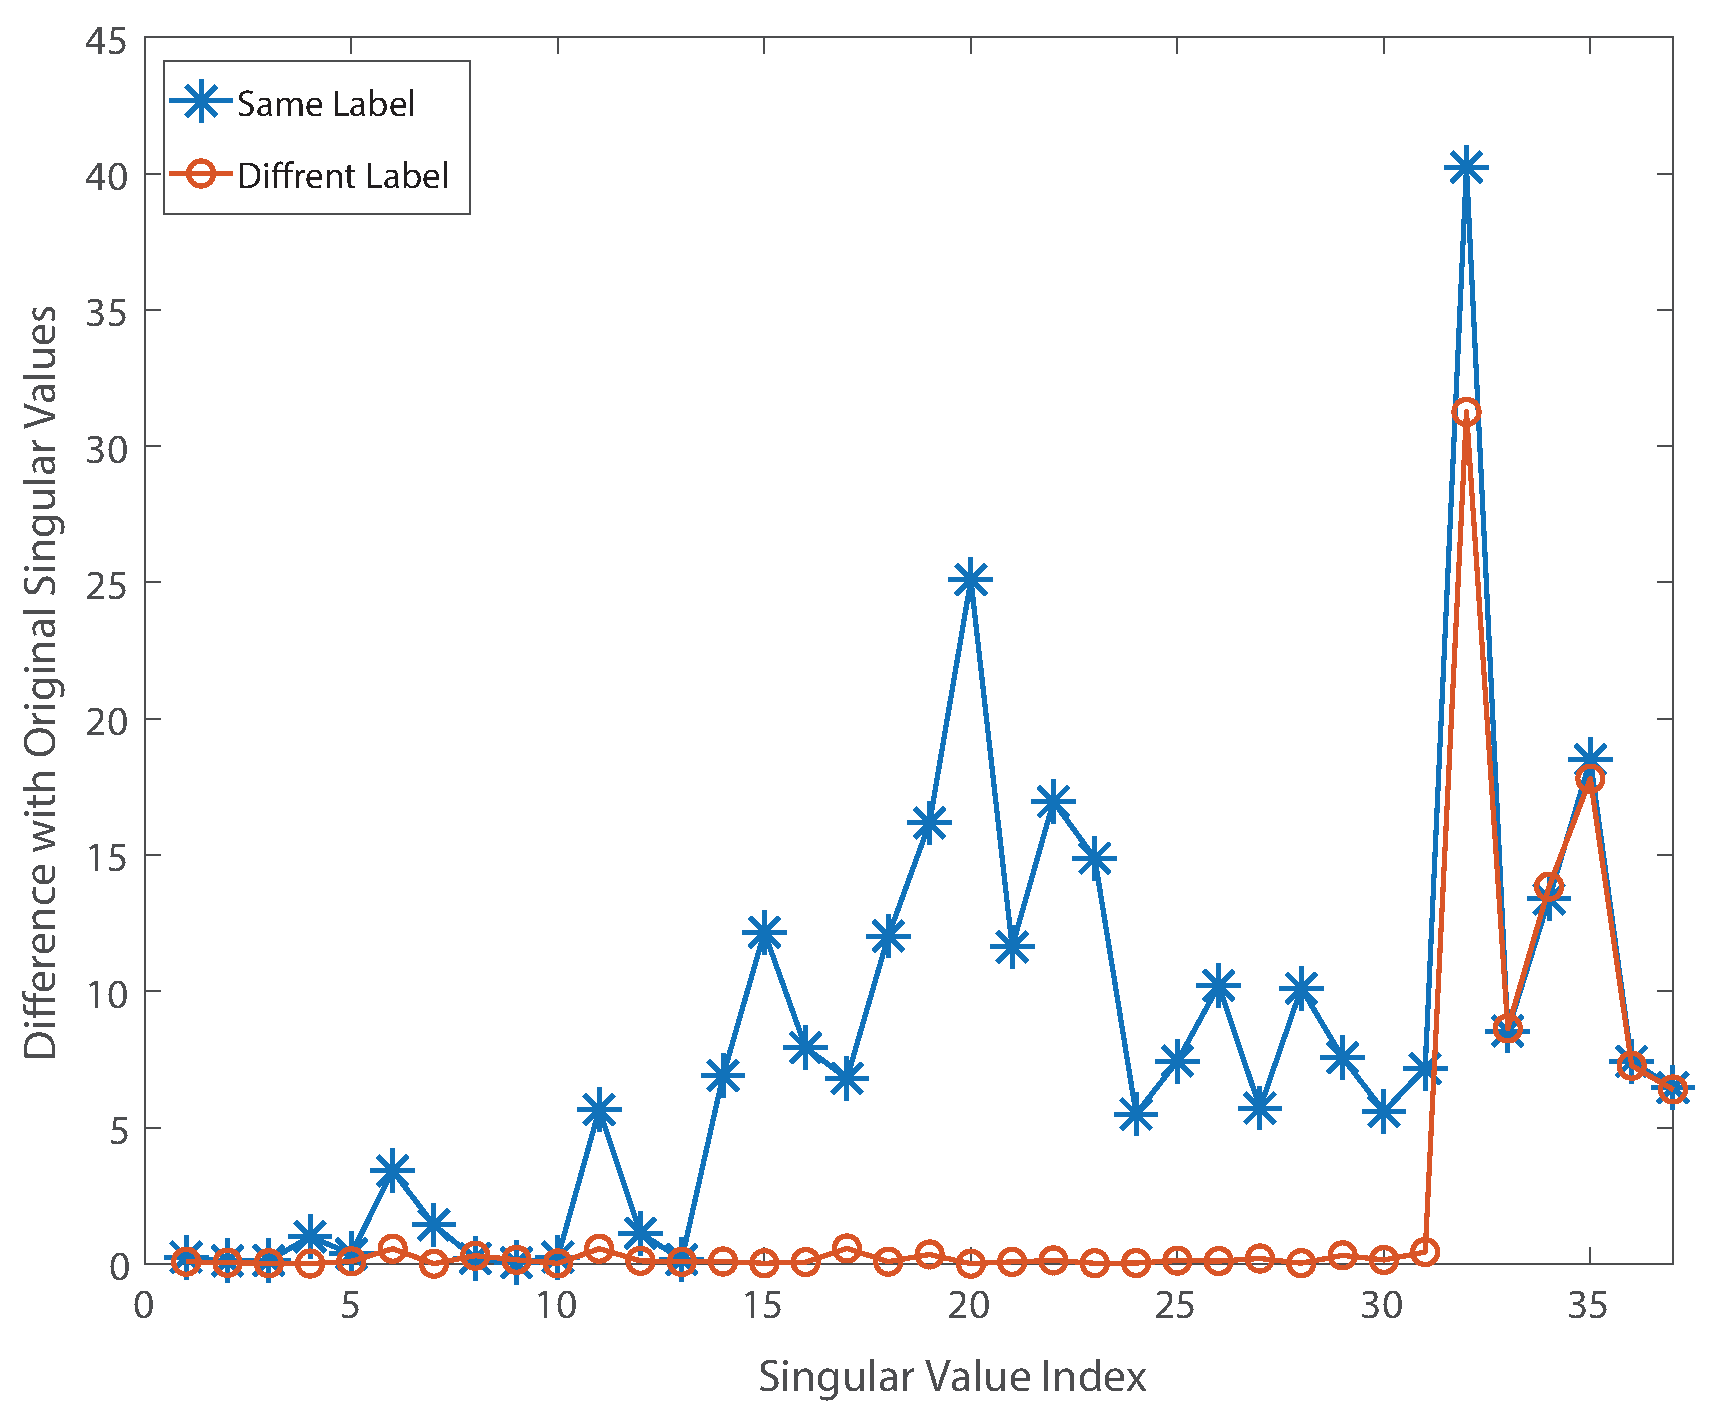
\includegraphics[width=3.5in]{images/SVDiff}
	%		\caption{The blue line with the star indicator, shows the difference between the mode-$3$ singular values of the original data and the data appended with a \emph{same} label subject. The orange line indicated with circles, shows the difference between the mode-$3$ singular values of the original data and the data appended with a \emph{different} label subject.}
	%		\label{g3.1}
	%	\end{figure}
	
	
	%As it was discussed before in \eqref{related_works}, there are two types of FC: Dynamic FC and Static FC. Although the obtained FC is an sFC by definition, we argue that the core tensor obtained from HOSVD, which contains the features included in the FC calculation process, has a dynamic structure. The majority of non-stationary methods uses the sliding window technique in order to analyze the BOLD signal in several sessions. The main idea is that the presence of temporal fluctuations in FC within different sessions should be taken into account in order to obtain a better FC.


	\section{EXPERIMENTAL STUDY}
	\subsection{Data Acquisition and Experimental Settings}
	
	Rs-fMRI data of $196$ subjects were downloaded from the ADNI website\footnote{http://adni.loni.usc.edu}. 
	44 eMCI and 38 NC subjects was obtained as it was in  \cite{r14}, except that the ROIs within the Cerebellum and Vermis are not excluded in our study. The IDs of the $82$ ($38$ NC and $44$ early MCI) subjects are provided in the supplementary material.
	
	
%	Rs-fMRI data of $196$ subjects were downloaded from the ADNI website\footnote{http://adni.loni.usc.edu}. Nine subjects were discarded
%	due to the corruption of data, and the remaining $187$ subjects were preprocessed for analysis. After removing subjects that had problems in the preprocessing steps, such as large head motion,
%	$156$ subjects were kept, including $26$ AD, $44$ early MCI, $38$ late MCI, $38$ NC, and ten significant memory concern labeled by ADNI. We used the $38$ NC and the $44$ early MCI because our focus in this paper is to identify MCI at a very early stage, which is the most challenging and significant task in AD
%	prediction. The IDs of the $82$ ($38$ NC and $44$ early MCI) subjects are provided in the supplementary material. 
%	
%	The data are acquired on a $3$-T (Philips) scanner with TR/TE set as $3000/30$
%	ms and flip angle of $80◦$. Each series has $140$ volumes, and each volume consists of 48 slices of image matrices with dimensions
%	$64 \times 64$
%	with voxel size of
%	$ 3.31 \times  3.31 \times 3.31$
%	$mm^3$ . The preprocessing is carried out using SPM12 and DPARSFA \cite{r64.5}. The
%	first ten volumes of each series are discarded for signal equilibrium. Slice timing, head motion correction, and MNI space normalization are performed. Participants with too much head motion are excluded. The normalized brain images are warped into automatic anatomical labeling (AAL) \cite{r64.7} atlas to obtain $116$ ROIs as nodes. By following common practice \cite{n1, n2, n3}, the ROI mean time series are extracted by averaging the time series from all voxels within each ROI and then bandpass filtered to obtain multiple sub-bands as in \cite{n3}. 
	
	
	

	
%	Nine subjects were discarded
%	due to the corruption of data, and the remaining $187$ subjects were preprocessed for analysis. After removing subjects that had problems in the preprocessing steps, such as large head motion,
%	$156$ subjects were kept, including $26$ AD, $44$ early MCI, $38$ late MCI, $38$ NC, and ten significant memory concern labeled by ADNI. We used the $38$ NC and the $44$ early MCI because our focus in this paper is to identify MCI at a very early stage, which is the most challenging and significant task in AD
%	prediction. The IDs of the $82$ ($38$ NC and $44$ early MCI) subjects are provided in the supplementary material. 
%	
%	The data are acquired on a $3$-T (Philips) scanner with TR/TE set as $3000/30$
%	ms and flip angle of $80◦$. Each series has $140$ volumes, and each volume consists of 48 slices of image matrices with dimensions
%	$64 \times 64$
%	with voxel size of
%	$ 3.31 \times  3.31 \times 3.31$
%	$mm^3$ . The preprocessing is carried out using SPM12 and DPARSFA \cite{r64.5}. The
%	first ten volumes of each series are discarded for signal equilibrium. Slice timing, head motion correction, and MNI space normalization are performed. Participants with too much head motion are excluded. The normalized brain images are warped into automatic anatomical labeling (AAL) \cite{r64.7} atlas to obtain $116$ ROIs as nodes. By following common practice, the ROI mean time series are extracted by averaging the time series from all voxels within each ROI and then bandpass filtered to obtain multiple sub-bands as in \cite{nn3}. 
	
	
	
	\subsection{Classification}
	
	Almost every subject in ADNI dataset has several scans. Usually, random scan data is selected and enters the processing step\cite{r14}. This random selection may cause several problems. Since the number of train data is very low, a small alteration in the samples could drastically change the set of input parameters in order to achieve the highest prediction accuracy and other classification evaluation methods. Also achieving high-quality results with a classifier does not guarantee its effectiveness on other datasets even with fine-tuning the parameters since the training set may contain outliers and unidentified corrupted data.
	
	In order to show that the proposed framework is less sensitive against the choice of different permutations of data (i.e. Same patient with the different scan), we have selected $18$ different permutations of data and test two state of the art \textbf{eMCI} classification methods on them: \textbf{HON}\cite{r14a} and \textbf{k-SICE}\cite{r14}.   
	To make full use of the limited subjects, a leave-one-out procedure is used for training and test. That is, each sample is reserved for the test in turn, while the remaining samples are used for training.
	We have use five
	evaluation measures: accuracy (ACC), sensitivity (SEN), Youden’s index(YI), F-score, and balanced accuracy (BAC).
	In this article, we treat the eMCI samples as positive class and the NC samples as negative class.
	%\begin{table}
	%	\begin{center}
	%			\caption{Definitions of five statistical measurement
	%			indices} \label{Table_1}
	%		\begin{tabular}{l c}
	%			\hline
	%			\hline
	%			Measureement & Definition\\
	%			\hline
	%			\\
	%			Acc & $\dfrac{TP+TN}{TP+FP+TN+FN}$\\[7pt]
	%			SEN & $\dfrac{TP}{TP+FN}$\\[7pt]
	%			%SPE & $\dfrac{TN}{TN+FP}$\\[7pt]
	%			YI & $SEN + SPE - 1$\\[7pt]
	%			F-Score & $2\times \dfrac{precesion \times recall}{precesion + recall}$\\[7pt]
	%			BAC & $\dfrac{1}{2}(SEN + SPE)$\\[7pt]
	%			\hline
	%			\hline
	%		\end{tabular}
	%	\end{center}
	%\end{table}
	
	
	\subsubsection{Classification performance}
	The classification accuracy measure(ACC), After fine-tuning the input parameter set for each method, show that for $16$ out of $18$ different random selected datasets, our approach performs better than k-SICE, the same also holds for $15$ datasets comparing to HON. i.e. in $88.8 \%$ of datasets, proposed method works better than k-SICE and in $83.3 \%$ of datasets, it works better than FON.  
	The highest classification accuracy($86.59\%$) is achieved with the proposed method in the $15$th sample data. The highest accuracy for the HON ($84.15\%$) is achieved in the $14$th, and the highest accuracy for the SICE method ($85.37\%$) is achieved in the $6$th sample data. As it was mentioned before, being stable when the input dataset changes is a very important aspect for a classifier, in order to measure the stability, the standard deviation of accuracy along with other measures are
	calculated. The std. of accuracy for the proposed method is $0.64$ times less than HON and $1.73$ times less than k-SICE method. Similar results also hold for other classification measures.
	\begin{figure*}
		\centering
		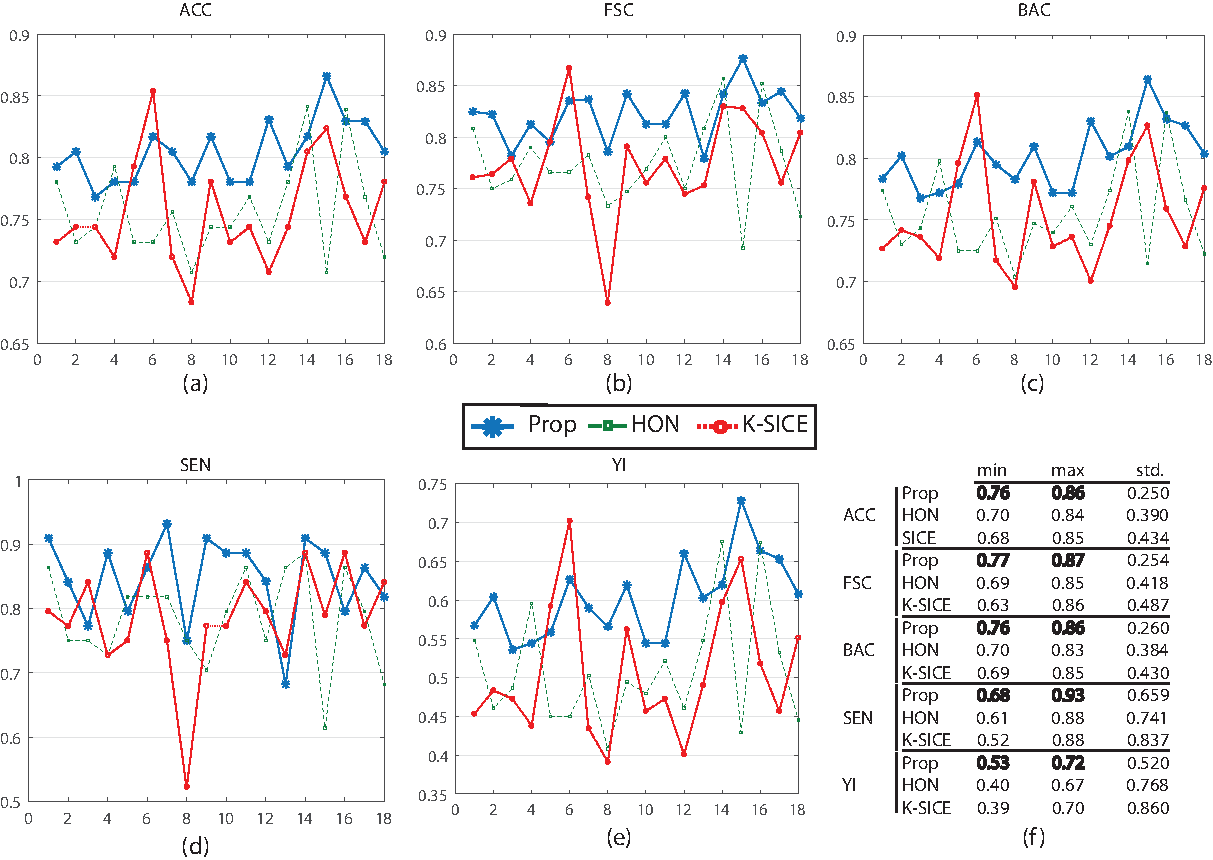
\includegraphics[width=6in]{images/Final-eps.pdf}
		\caption{
			% Updated upstream
			Comparison of proposed method(Prop) with K-SICE and HON 
			applied on 18 different dataset permutations 
			in five different classification evaluation measures.
			Figures \textit{a} through \textit{e} show \textit{accuracy}, \textit{F-Score}, \textit{balanced accuracy}, \textit{sensitivity} and \textit{Youden Index} respectively
			along with the max, min and standard deviation of each one presented at the embedded table (f). 
			%=======
			%		Comparison of proposed method(Prop) with K-SICE and HON in five different classification evaluation measures along with the standard deviation of each one. %As it can be seen, the both the minimum and maximum of the proposed methods in these measurements are higher that the other two. Also the lower std. of our method indicates its stability.   
			%>>>>>>> Stashed changes
		}
		\label{g3.2}
	\end{figure*}
	
	
	Figure \eqref{g3.2} show the performance of these three methods in all five measurements. Some statistical information about these plots is also included in the embedded table. As it can be seen in this figure, similar to the accuracy, the proposed method in overall works much better than HON and k-SICE. For a better Demonstration, table \eqref{AVG} provides the average of several classification measurements scores for all dataset permutations. 
	\begin{table}
		\begin{center}
			\caption{The Average of Different Classification Measurements in all dataset permutations in \% }
			%\resizebox{\textwidth}{!}{  
			\begin{tabular}{@{}c*{6}{c}}
				\hline\hline
				Method&ACC& F-Score&SEN & SPE &YI & BAC 
				\\
				\hline
				k-SICE  &75.57& 77.36 & 78.50 & 72.19 & 50.69 & 75.34 
				\\
				HON   &75.66& 77.44 & 78.40 & 72.48 & 50.89 & 75.44  
				\\
				Proposed &\textbf{80.43}& \textbf{82.20} & \textbf{84.60} & \textbf{75.59} & \textbf{60.20} & \textbf{80.09}
				
				\\
				
				\hline\hline
				\label{AVG}
			\end{tabular}
			%}
		\end{center}
	\end{table}
	As it can be seen in this table, the average accuracy of Proposed method which is $80.43 \%$ is $4.77\%$ higher than the next method HON, and $4.86 \%$ better than k-SICE. It is noteworthy that The other two methods i.e HON and SICE show similar results in average.  
	
	\begin{figure*}
		\centering
		
\includegraphics[width=6in]{images/FG}
		\caption{
			The difference graph. This graph is obtained via subtracting the functional connectivity of eMCI subjects from normal subjects. Each circle represents a ROI in AAL atlas and the color and size of each circle is proportional to the graph clustering coefficient of the difference graph. red = more activity in EMCI, green: less. 
		}
		\label{g3.3}
	\end{figure*}
	
	One other key aspect of the proposed classifier is that it works significantly faster that the other two, specially in the training process. Our method is more than $600$ times faster than HON and $20$ times faster that SICE. Having a huge execution time especially affects the parameter selection for HON, since it uses cross-validation procedure in order to find the optimal parameters which itself require several runs of the algorithm.   
	
	
%	\subsubsection{Runtime Comparison}
%	One other key features of the proposed method is that it works significantly faster than the other two methods. Table \eqref{Time} shows the average elapsed time (Training plus Testing) of each method for all data permutations. These methods were executed in Matlab R2017b and carried with an Intel Core-i7 processor and $16$GB of RAM. As it can be seen in this table, the proposed method is more than $600$ times faster than HON and $20$ times faster that SICE.   
%	\begin{table}
%		\begin{center}
%			\caption{Elapsed time of the test and train phase in seconds}
%			%\resizebox{\textwidth}{!}{  
%			\begin{tabular}{@{}c*{4}{c}}
%				\hline\hline
%				Method& HON & k-SICE& proposed method 
%				\\
%				\hline
%				Elapsed Time  &6950& 230 & 11 
%				\\
%				\hline\hline
%				\label{Time}
%			\end{tabular}
%			%}
%		\end{center}
%	\end{table}
%	Having a huge execution time especially affects the parameter selection for HON, since it uses cross-validation procedure in order to find the optimal parameters which itself require several runs of the algorithm. 
%
%	
	
	
	\subsection{Functional connectivity Network}
		The vector features for both Normal and eMCI classes was obtained via the proposed method as it is described in \eqref{FC_Construction}. Due to the aforementioned qualities of partial correlation, SICE is deployed in order to obtain the final FC.  
	In order to better highlight the differences between Normal and eMCI subjects, a difference graph $D$ is constructed by subtracting the Normal FC from the eMCI FC. This graph could be seen in Figure\eqref{g3.3}. 
	The nodes of $D$ shows the ROIs according to the AAL atlas. The size of each node is proportional to its graph clustering coefficient, i.e. the bigger node demonstrates higher activity in eMCI subjects in the corresponding ROI. 
	Similar to nodes, the size of each edge is also proportional to the correlation between two ROIs. In addition, the edges are also color-coded in a way that the green edges show the positive edges in $D$ and the red edges show the negative edges in $D$. In this manner, the green edges demonstrate decreasing in activity between the corresponding nodes in eMCI subjects and vice versa, the red edges show increasing activity between corresponding ROIs in the eMCI subjects.   
	
	As it can be seen in the difference graph, the big nodes i.e. ROIs with higher activities does not necessarily establish strong connections with the other nodes. As an obvious example, higher activities in Lingual gyrus(ROI index: 47,48)\cite{r25}, Calcarine sulcus(ROI index: 43, 44)\cite{r26,r27}, Supplementary motor area(ROI index: 19,20)\cite{r27,r28} and Temporal\_mid\_L(ROI index: 85)\cite{r29} are easily detectable. The majority of ROIs located in frontal lobe also shows rather high activities comparing to normal subjects\cite{r30,r04}.
	
	Similar to the nodes, the strong edge between two ROIs does not necessarily require the nodes to be highly active in eMCI. Although a strong edge does indicate high activities and functional connectivity between the two corresponding ROIs. The difference Graph shows a significant increase in connectivity between 
	Rectus(ROI index: 28, 27 in Frontal lobe) and 
	Parietal\_Sup\_R(ROI index: 60 in Parietal lobe) \cite{r40, r41},
	Frontal\_Inf\_Orb\_R(ROI index: 16 in Frontal lobe) and
	Cingulum\_Ant(ROI index: 31,32 in Limbic lobe)\cite{r42},
	Insula\_L, Temporal\_Pole\_Sup\_L(ROI index: 29,83 in Limbic lobe) and
	Pallidum\_R, Caudate\_R(ROI index: 29,83 in Sub Cortical Grey Nuclei)\cite{r43}. It can also be seen that within activities in frontal lobe also increased in patients with eMCI\cite{r44}. There is a decrease in connectivity between Amygdala\_L(ROI index: 41 in Sub Cortical Grey Nuclei) with Frontal\_Mid\_Orb\_R(ROI index: 10 in Sub Frontal lobe) and ParaHippocampal\_L(ROI index: 39 in Sub Limbic lobe)\cite{r45}. The connectivity between Heschl\_L(ROI index: 79 in Temporal lobe) and two ROIs Temporal\_Mid\_R(ROI index: 86 also in Temporal lobe) and Occipital\_Inf\_R(ROI index: 54 in Occipital lobe) also decreased in eMCI\cite{r46}. 
	
	\subsubsection*{\textbf{Regarding the Cerebellum and Vermis}}
	In fMRI data analysis and especially in Alzheimer's disease studies, ROIs within the Cerebellum and Vermis are usually excluded since their role was regarded as insignificant\cite{r47, r48}. Recent studies have shown that the traditional assumption that Cerebral area is essential only for the coordination of voluntary motor activity and motor learning is not valid and indicates the significant role of the cerebellum in nervous system function, cognition, and emotion\cite{r32}. 
	
	As it can be seen in the difference graph that we obtained, ROIs within Cerebellum and Vermis are highly active and both their Intra and interconnections are noticeable. There is increased functional connectivity between the Limbic lobe especially 
	Hippocampus\_R, Temporal\_Pole\_Mid(ROI index: 38,87,88)
	and Cerebral areas in eMCI patients. Also, the connectivity between Occipital lobe, especially Occipital\_mid\_R(ROI index: 52), the Frontal lobe, especially in Frontal\_mid\_orb(ROI index: 9,10) and Cerebral areas seems to decrease in patients with eMCI. 
	
	
	
	
	%\begin{table*}
	%	\begin{center}
	%		\caption{Active Nodes }
	%		\resizebox{\textwidth}{!}{  
	%		\begin{tabular}{@{}l*{4}{l}}
	%			\hline\hline
	%			NO.&ROI Index&ROI name&Location& Citations 
	%			\\
	%			\hline
	%			1& 8 & Frontal\_Mid\_R & Middle frontal gyrus
	%			$\rightarrow$ Prefrontal cortex $\rightarrow$ \textbf{Frontal lobe}
	%			 & Main 
	%			\\
	%			2& 14 & Frontal\_Inf\_Tri\_R & Inferior frontal gyrus, pars triangularis
	%			$\rightarrow$ Inferior frontal gyrus $\rightarrow$ Prefrontal cortex
	%			 $\rightarrow$ \textbf{Frontal lobe} & Main 
	%			\\
	%			3& 17 & Rolandic\_Oper\_L & Rolandic operculum
	%			$\rightarrow$ Operculum $\rightarrow$ \textbf{Cerebral cortex} & Main 
	%			\\
	%			4& 19 & Supp\_Motor\_Area\_L & Supplementary motor area
	%			$\rightarrow$ Motor area $\rightarrow$ \textbf{Functional area} & Main 
	%			\\
	%			5& 20 & Supp\_Motor\_Area\_R & Supplementary motor area
	%			$\rightarrow$ Motor area $\rightarrow$ \textbf{Functional area} & Main 
	%			\\
	%			6& 25 & Frontal\_Med\_Orb\_L &  Medial orbitofrontal cortex $\rightarrow$ Orbitofrontal cortex
	%			$\rightarrow$ Orbitofrontal area $\rightarrow$ \textbf{Frontal lobe} & ? 
	%			\\
	%			7 & 34 & Cingulum\_Mid\_R & Right midcingulate area
	%			$\rightarrow$ Midcingulate area $\rightarrow$ Cingulate gyrus
	%			$\rightarrow$ Cerebral cortex $\rightarrow$ \textbf{Frontal lobe} & ? 
	%			\\
	%			8 & 43 & Calcarine\_L & Calcarine sulcus
	%			$\rightarrow$ Midcingulate area $\rightarrow$ \textbf{Sulcus} & ? 
	%			\\
	%			9 & 44 & Calcarine\_R & Calcarine sulcus
	%			$\rightarrow$ Midcingulate area $\rightarrow$ \textbf{Sulcus} & ? 
	%			\\
	%			10 & 47 & Lingual\_L & Lingual gyrus
	%			$\rightarrow$ Occipital lobe $\rightarrow$Cerebral cortex $\rightarrow$ \textbf{Frontal lobe} & ? 
	%			\\
	%			11 & 48 & Lingual\_R & Lingual gyrus
	%			$\rightarrow$ Occipital lobe $\rightarrow$Cerebral cortex $\rightarrow$ \textbf{Frontal lobe} & ? 
	%			\\
	%			12 & 70 & Paracentral\_Lobule\_R & Paracentral lobule $\rightarrow$ \textbf{Frontal lobe} & ?
	%			\\
	%			13 & 69 & Paracentral\_Lobule\_L & Middle temporal gyrus $\rightarrow$ \textbf{Temporal lobe} & ?
	%			\\
	%			14 & 99 & Cerebelum\_6\_L & Lobule VI of cerebellar hemisphere $\rightarrow$Cerebellum
	%			$\rightarrow$ Metencephalon $\rightarrow$ \textbf{Hindbrain} & ?
	%			\\
	%			15 & 111 & Vermis\_4\_5 & Vermis $\rightarrow$ Cerebellum $\rightarrow$ Metencephalon $\rightarrow$ \textbf{Hindbrain} & ?
	%			\\
	%			\hline\hline
	%			\label{sss}
	%		\end{tabular}
	%		}
	%	\end{center}
	%\end{table*}
	
	
	
	
	% An example of a floating figure using the graphicx package.
	% Note that \label must occur AFTER (or within) \caption.
	% For figures, \caption should occur after the \includegraphics.
	% Note that IEEEtran v1.7 and later has special internal code that
	% is designed to preserve the operation of \label within \caption
	% even when the captionsoff option is in effect. However, because
	% of issues like this, it may be the safest practice to put all your
	% \label just after \caption rather than within \caption{}.
	%
	% Reminder: the "draftcls" or "draftclsnofoot", not "draft", class
	% option should be used if it is desired that the figures are to be
	% displayed while in draft mode.
	%
	%\begin{figure}[!t]
	%\centering
	%\includegraphics[width=2.5in]{myfigure}
	% where an .eps filename suffix will be assumed under latex, 
	% and a .pdf suffix will be assumed for pdflatex; or what has been declared
	% via \DeclareGraphicsExtensions.
	%\caption{Simulation results for the network.}
	%\label{fig_sim}
	%\end{figure}
	
	% Note that the IEEE typically puts floats only at the top, even when this
	% results in a large percentage of a column being occupied by floats.
	
	
	% An example of a double column floating figure using two subfigures.
	% (The subfig.sty package must be loaded for this to work.)
	% The subfigure \label commands are set within each subfloat command,
	% and the \label for the overall figure must come after \caption.
	% \hfil is used as a separator to get equal spacing.
	% Watch out that the combined width of all the subfigures on a 
	% line do not exceed the text width or a line break will occur.
	%
	%\begin{figure*}[!t]
	%\centering
	%\subfloat[Case I]{\includegraphics[width=2.5in]{box}%
	%\label{fig_first_case}}
	%\hfil
	%\subfloat[Case II]{\includegraphics[width=2.5in]{box}%
	%\label{fig_second_case}}
	%\caption{Simulation results for the network.}
	%\label{fig_sim}
	%\end{figure*}
	%
	% Note that often IEEE papers with subfigures do not employ subfigure
	% captions (using the optional argument to \subfloat[]), but instead will
	% reference/describe all of them (a), (b), etc., within the main caption.
	% Be aware that for subfig.sty to generate the (a), (b), etc., subfigure
	% labels, the optional argument to \subfloat must be present. If a
	% subcaption is not desired, just leave its contents blank,
	% e.g., \subfloat[].
	
	
	% An example of a floating table. Note that, for IEEE style tables, the
	% \caption command should come BEFORE the table and, given that table
	% captions serve much like titles, are usually capitalized except for words
	% such as a, an, and, as, at, but, by, for, in, nor, of, on, or, the, to
	% and up, which are usually not capitalized unless they are the first or
	% last word of the caption. Table text will default to \footnotesize as
	% the IEEE normally uses this smaller font for tables.
	% The \label must come after \caption as always.
	%
	%\begin{table}[!t]
	%% increase table row spacing, adjust to taste
	%\renewcommand{\arraystretch}{1.3}
	% if using array.sty, it might be a good idea to tweak the value of
	% \extrarowheight as needed to properly center the text within the cells
	
	
	
	
	
	
	
	
	
	
	
	
	
	
	
	
	
	
	
	
	
	
	
	
	%\caption{An Example of a Table}
	%\label{table_example}
	%\centering
	%% Some packages, such as MDW tools, offer better commands for making tables
	%% than the plain LaTeX2e tabular which is used here.
	%\begin{tabular}{|c||c|}
	%\hline
	%One & Two\\
	%\hline
	%Three & Four\\
	%\hline
	%\end{tabular}
	%\end{table}
	
	
	% Note that the IEEE does not put floats in the very first column
	% - or typically anywhere on the first page for that matter. Also,
	% in-text middle ("here") positioning is typically not used, but it
	% is allowed and encouraged for Computer Society conferences (but
	% not Computer Society journals). Most IEEE journals/conferences use
	% top floats exclusively. 
	% Note that, LaTeX2e, unlike IEEE journals/conferences, places
	% footnotes above bottom floats. This can be corrected via the
	% \fnbelowfloat command of the stfloats package.
	
	
	
	
	
	\section{Conclusion}
	The majority of classification techniques uses the vectorized version of data as the input of the discriminant function. As the number of the dimensions grows, i.e. when data is naturally a high order tensor, this vectorization become problematic and it would highly affect the  performance. Taking advantage of the techniques designed for the tensors, we have developed a framework for fMRI data analysis in which the following objectives: 
\textit{Classification} 
		and
		\textit{General Functional Connectivity network}
	are achieved via a singe HOSVD of the input tensors. 
	
	Extensive studies on the rs-fMRI provided by ADNI shows the superiority of the proposed framework in both classification and functional connectivity. The obtained FC network not only acknowledge the previous discovered connections but also reveals new connectivity patterns previously unknown.
	The framework proposed in this paper can be easily extended to other studies involved with high order data.  
	
	%\begin{table*}
	%	\begin{center}
	%		\caption{content...}
	%		\resizebox{\textwidth}{!}{  
	%	\begin{tabular}{@{}c*{20}{c}}
	%		\hline\hline
	%		\multicolumn{20}{c}{Datasets} 
	%		\\
	%		\hline
	%&\multicolumn{1}{|c}{TBNA} & \textbf{79.27} & \textbf{80.49} & \textbf{76.83} & 78.05 & 78.05 & 81.71 & \textbf{80.49} & \textbf{78.05} & \textbf{81.71} & \textbf{78.05} & \textbf{78.05} & \textbf{83.1} & \textbf{79.27} & 8171 & \textbf{86.59} & 82.93 & \textbf{82.93} & \textbf{80.49} 
	%\\
	%ACC&\multicolumn{1}{|c}{FON} & 78.05 & 73.17 & 74.39 & \textbf{79.27} & 73.17 & 73.17 & 75.61 & 70.73 & 74.39 & 74.39 & 76.83 & 73.17 & 78.05 & \textbf{84.15} & 70.73 & \textbf{83.9} & 76.83 & 71.95 
	%\\
	%&\multicolumn{1}{|c}{SICE} & 73.17 & 74.39 & 74.39 & 71.95 & \textbf{79.27} & \textbf{85.37} & 71.95 & 68.29 & 78.05 & 73.17 & 74.39 & 70.73 & 74.39 & 80.49 & 82.38 & 76.83 & 73.17 & 78.05 
	%%\\\hline
	%%&\multicolumn{1}{|c}{TBNA} & \textbf{0.9091} & \textbf{0.8409} & 0.7727 & \textbf{0.8864} & 0.7955 & \textbf{0.8636} & \textbf{0.9318} & 0.75 & \textbf{0.9091} & \textbf{0.8864} & \textbf{0.8864} & \textbf{0.8421} & 0.6818 & \textbf{0.9091} & \textbf{0.8864} &\textbf{ 0.7955} &\textbf{ 0.8636} & \textbf{0.8182} 
	%%\\
	%%SEN&\multicolumn{1}{|c}{FON} & 0.8636 & 0.75 & 0.75 & 0.7273 & \textbf{0.8182} & 0.8182 & 0.8182 & 0.75 & 0.7045 & 0.7955 & 0.8636 & 0.75 & \textbf{0.8636} & 0.8864 & 0.6136 & 0.8636 & 0.7955 & 0.6818 
	%%\\
	%%&\multicolumn{1}{|c}{SICE} & 0.7955 & 0.7727 & \textbf{0.8409} & 0.7273 & 0.75 & 0.8864 & 0.75 & 0.5227 & 0.7727 & 0.7727 & 0.8409 & 0.7955 & 0.7273 & 0.8864 & 0.7895 & 0.8864 & 0.7727 & 0.8409 
	%\\\hline
	%%&\multicolumn{1}{|c}{TBNA} & 0.6579 & \textbf{0.7632} & \textbf{0.7632} & 0.6579 & \textbf{0.7632} & 0.7632 & 0.6579 & 0.8158 & 0.7105 & 0.6579 & 0.6579 & 0.8182 & 0.9211 & 0.7105 & 0.8421 & 0.8684 & 0.7895 & 0.7895 
	%%\\
	%%SPE&\multicolumn{1}{|c}{FON} & 0.6842 & 0.7105 & 0.7368 & 0.8684 & 0.6316 & 0.6316 & 0.6842 & 0.6579 & 0.7895 & 0.6842 & 0.6579 & 0.7105 & 0.6842 & 0.7895 & 0.8158 & 0.8106 & 0.7368 & 0.7632 
	%%\\
	%%&\multicolumn{1}{|c}{SICE} & 0.6579 & 0.7105 & 0.6316 & 0.7105 & 0.8421 & 0.8158 & 0.6842 & 0.8684 & 0.7895 & 0.6842 & 0.6316 & 0.6053 & 0.7632 & 0.7105 & 0.8636 & 0.6316 & 0.6842 & 0.7105 
	%%\\\hline
	%%&\multicolumn{1}{|c}{TBNA} & 0.567 & 0.6041 & 0.5359 & 0.5443 & 0.5586 & 0.6268 & 0.5897 & 0.5658 & 0.6196 & 0.5443 & 0.5443 & 0.6603 & 0.6029 & 0.6196 & 0.7285 & 0.6639 & 0.6531 & 0.6077 
	%%\\
	%%YI&\multicolumn{1}{|c}{FON} & 0.5478 & 0.4605 & 0.4868 & 0.5957 & 0.4498 & 0.4498 & 0.5024 & 0.4079 & 0.494 & 0.4797 & 0.5215 & 0.4605 & 0.5478 & 0.6758 & 0.4294 & 0.6742 & 0.5323 & 0.445 
	%%\\
	%%&\multicolumn{1}{|c}{SICE} & 0.4533 & 0.4833 & 0.4725 & 0.4378 & 0.5921 & 0.7022 & 0.4342 & 0.3911 & 0.5622 & 0.4569 & 0.4725 & 0.4007 & 0.4904 & 0.5969 & 0.6531 & 0.5179 & 0.4569 & 0.5514 
	%%\\\hline
	%&\multicolumn{1}{|c}{TBNA} &\textbf{ 82.47} & \textbf{82.22} & \textbf{78.16} & \textbf{81.25} & \textbf{79.55} & 83.52 & \textbf{83.67} &\textbf{ 78.57} & \textbf{84.21} & \textbf{81.25 } & \textbf{81.25} & \textbf{84.25} & 77.92 & 84.21 & \textbf{87.64 }& 83.33 & \textbf{84.44} & \textbf{81.82 }
	%\\
	%F-SC&\multicolumn{1}{|c}{FON} & 80.85 & 75 & 75.86 & 79.01 & 76.6 & 76.6 & 78.26 & 73.33 & 74.7 & 76.92 & 80 & 75 & \textbf{80.85} & \textbf{85.71} & 69.23 & \textbf{85.2} & 78.65 & 72.29 
	%\\
	%&\multicolumn{1}{|c}{SICE} & 76.09 & 76.4 & 77.89 & 73.56 & 79.52 & \textbf{86.67} & 74.16 & 63.89 & 79.07 & 75.56 & 77.89 & 74.47 & 75.29 & 82.98 & 82.79 & 80.41 & 75.56 & 80.43 
	%\\\hline
	%%&\multicolumn{1}{|c}{TBNA} & 0.7835 & 0.802 & 0.7679 & 0.7721 & 0.7793 & 0.8134 & 0.7949 & 0.7829 & 0.8098 & 0.7721 & 0.7721 & 0.8301 & 0.8014 & 0.8098 & 0.8642 & 0.8319 & 0.8266 & 0.8038 
	%%\\
	%%BAC&\multicolumn{1}{|c}{FON} & 0.7739 & 0.7303 & 0.7434 & 0.7978 & 0.7249 & 0.7249 & 0.7512 & 0.7039 & 0.747 & 0.7398 & 0.7608 & 0.7303 & 0.7739 & 0.8379 & 0.7147 & 0.8371 & 0.7661 & 0.7225 
	%%\\
	%%&\multicolumn{1}{|c}{SICE} & 0.7267 & 0.7416 & 0.7362 & 0.7189 & 0.7961 & 0.8511 & 0.7171 & 0.6956 & 0.7811 & 0.7285 & 0.7362 & 0.7004 & 0.7452 & 0.7984 & 0.8266 & 0.759 & 0.7285 & 0.7757 
	%%		& HON & &\multicolumn{1}{|c}{kernel} & \\
	%%		
	%%		& TBNA & &\multicolumn{1}{|c}{kernel} & \\
	%		 \\
	%		\hline\hline
	%	\end{tabular}
	%}
	%	\end{center}
	%\end{table*}
	
	
	
	
	
	
	
	% if have a single appendix:
	%\appendix[Proof of the Zonklar Equations]
	% or
	%\appendix  % for no appendix heading
	% do not use \section anymore after \appendix, only \section*
	% is possibly needed
	
	% use appendices with more than one appendix
	% then use \section to start each appendix
	% you must declare a \section before using any
	% \subsection or using \label (\appendices by itself
	% starts a section numbered zero.)
	%
	
	
	%\appendices
	%\section{Proof of the First Zonklar Equation}
	%Appendix one text goes here.
	
	% you can choose not to have a title for an appendix
	% if you want by leaving the argument blank
	%\section{}
	%Appendix two text goes here.
	
	
%	% use section* for acknowledgment
%	\section*{Acknowledgment}
%	
%	
%	The authors would like to thank...
	
	
	% Can use something like this to put references on a page
	% by themselves when using endfloat and the captionsoff option.
	\ifCLASSOPTIONcaptionsoff
	\newpage
	\fi
	
	
	
	% trigger a \newpage just before the given reference
	% number - used to balance the columns on the last page
	% adjust value as needed - may need to be readjusted if
	% the document is modified later
	%\IEEEtriggeratref{8}
	% The "triggered" command can be changed if desired:
	%\IEEEtriggercmd{\enlargethispage{-5in}}
	
	% references section
	
	% can use a bibliography generated by BibTeX as a .bbl file
	% BibTeX documentation can be easily obtained at:
	% http://mirror.ctan.org/biblio/bibtex/contrib/doc/
	% The IEEEtran BibTeX style support page is at:
	% http://www.michaelshell.org/tex/ieeetran/bibtex/
	%\bibliographystyle{IEEEtran}
	% argument is your BibTeX string definitions and bibliography database(s)
	%\bibliography{IEEEabrv,../bib/paper}
	%
	% <OR> manually copy in the resultant .bbl file
	% set second argument of \begin to the number of references
	% (used to reserve space for the reference number labels box)




\bibliographystyle{IEEEtran}

\bibliography{aliref}
	% biography section
	% 
	% If you have an EPS/PDF photo (graphicx package needed) extra braces are
	% needed around the contents of the optional argument to biography to prevent
	% the LaTeX parser from getting confused when it sees the complicated
	% \includegraphics command within an optional argument. (You could create
	% your own custom macro containing the \includegraphics command to make things
	% simpler here.)
	%\begin{IEEEbiography}[{\includegraphics[width=1in,height=1.25in,clip,keepaspectratio]{mshell}}]{Michael Shell}
	% or if you just want to reserve a space for a photo:
	
%	\begin{IEEEbiography}{Mansoor Rezghi}
%		
%	\end{IEEEbiography}
%	
%	\begin{IEEEbiography}{Ali Noroozi}
%		
%	\end{IEEEbiography}
	
	% if you will not have a photo at all:
	%	\begin{IEEEbiographynophoto}{Mansoor Rezghi}
	%		
	%	\end{IEEEbiographynophoto}
	
	% insert where needed to balance the two columns on the last page with
	% biographies
	%\newpage
	
	%\begin{IEEEbiographynophoto}{Mansoor Rezghi}
	%Biography text here.
	%\end{IEEEbiographynophoto}
	
	% You can push biographies down or up by placing
	% a \vfill before or after them. The appropriate
	% use of \vfill depends on what kind of text is
	% on the last page and whether or not the columns
	% are being equalized.
	
	%\vfill
	
	% Can be used to pull up biographies so that the bottom of the last one
	% is flush with the other column.
	%\enlargethispage{-5in}
	
	
	
	% that's all folks
\end{document}







% The feature extraction methods are: \textbf{Naive Vectorization(NV):} which is the vectorized raw samples, \textbf{SICE Vectorized(SICE-V):} the vectorization of SICE matrices, \textbf{TBNA Vectorized(TBNA-V):} the vectorization of TBNA matrices, \textbf{SLR Vectorized(SLR-V):} the vectorization of SLR matrices, \textbf{SICE} and \textbf{TBNA} 